\chapter{The communication potential of FET projects on quantum technologies}
As shown in chapter \ref{FET_projects_and_social_media}, FET research projects on quantum technologies make limited use of online communication channels. In particular, none of them has considered the creation of an account on Twitter, the most common social platform among FET initiatives. It is therefore interesting to estimate the community which could be reached by QT projects via Twitter.

To this aim, the following analysis was performed. First, two hashtags likely to identify tweets related to QT were monitored over disparate periods of time. The same was repeated for two hashtags related to HPC. HPC was chosen   
 
Lorem ipsum dolor sit amet, consectetur adipisci elit, sed eiusmod tempor incidunt ut labore et dolore magna aliqua. Ut enim ad minim veniam, quis nostrum exercitationem ullam corporis suscipit laboriosam, nisi ut aliquid ex ea commodi consequatur. Quis aute iure reprehenderit in voluptate velit esse cillum dolore eu fugiat nulla pariatur. Excepteur sint obcaecat cupiditat non proident, sunt in culpa qui officia deserunt mollit anim id est laborum.

Data shown in this chapter was collected with the Twitter Analytics Tool Twitonomy. 

\section{QT Hashtag performance}
Two hashtags were monitored to assess of the reach potential of FET projects on QTs. These were \#quantumcomputing and the application of the AND logic operator to \#quantum and \#technology. 

Both analyses covered two periods of time. For \#quantumcomputing, the two periods were from 7th to 14th and from 20th to 25th October 2017, respectively. Those for the combination \#quantum AND \#technology spanned the time intervals between 4th and 14th and between 15th and 25th October 2017. The time periods were chosen randomly and based on the day ranges available to Twitonomy for the considered volume of tweets. Different choices of the time periods would not change significantly the estimates presented in this chapter.  

The distribution of the number of Tweets presenting the hashtags \#quantumcomputing and the combination \#quantum AND \#technology over the considered periods are shown in figures \ref{First-SecondSearch_QuantumComputing} and \ref{First-SecondSearch_QuantumTechnology}. The plots show that, typically, hundreds of tweets with the hashtag \#quantumcomputing are posted daily, whereas few show both hashtags \#quantum and \#technology. 

The potential reach of FET projects on QTs is summarised by data in Tables \ref{Summary_QuantumComputing-Technology}. Things are discussed in section ... .

\begin{table}[t]
 \begin{center}
 
  \begin{tabular}{cccc}
   \hline 
   \hline
   \multicolumn{4}{c}{\#quantumcomputing}\\
   \hline
   \hline
   Time period & Tweets & Users & Potential Reach \\ 
   \hline
   7 - 14 Oct 2017 & 1 928 & 1 270 & 9 392 166  \\
   20 - 25 Oct 2017 & 2 563 & 1 738 & 10 604 445  \\
   \hline
   \hline
  \end{tabular}

  \bigskip

  \begin{tabular}{cccc}
   \hline 
   \hline
   \multicolumn{4}{c}{\#quantum AND \#technology}\\
   \hline 
   \hline
   Time period & Tweets & Users & Potential Reach \\ 
   \hline
   4 - 14 Oct 2017 & 79 & 75 & 280 849  \\
   15 - 25 Oct 2017 & 36 & 28 & 85 123  \\
   \hline
   \hline
  \end{tabular}
 \end{center} 
 \caption{Summary of the Twitter analytics for the hashtag combination \#quantum AND \#technology over the two monitored time periods. The potential reach is defined as the total aggregate number of followers of the people who mentioned the considered keyword in their tweets.}
\label{Summary_QuantumComputing-Technology} 
\end{table}    

\begin{figure}
 \centering
 \begin{subfigure}[b]{0.9\textwidth}
   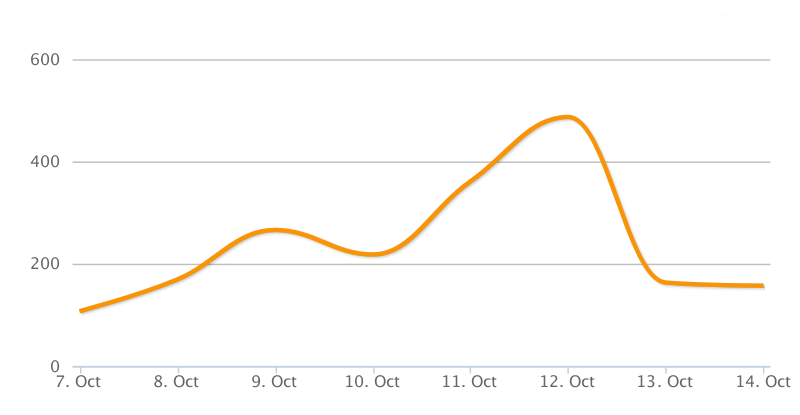
\includegraphics[width=1\linewidth]{Images/FirstSearch_QuantumComputing.png}
   \caption{} 
 \end{subfigure}

 \begin{subfigure}[b]{0.9\textwidth}
   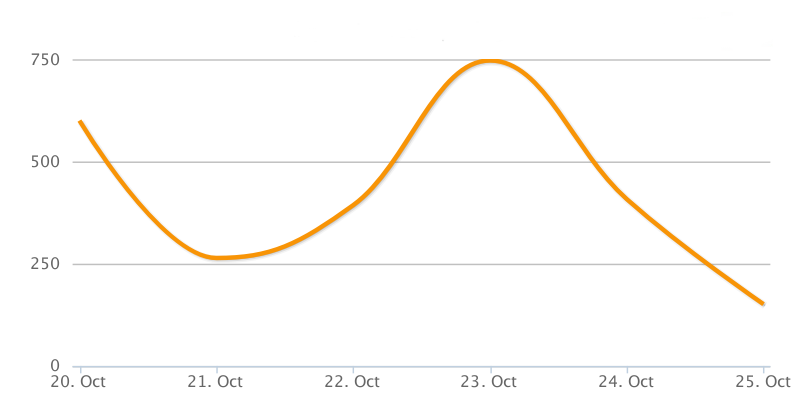
\includegraphics[width=1\linewidth]{Images/SecondSearch_QuantumComputing.png}
   \caption{}
 \end{subfigure}
 \caption{(a) Number of tweets with hashtag \#quantumcomputing posted between 7th and 14th October 2017. (b) As for (a) but over the time period between 20th and 25th October 2017.} 
 \label{First-SecondSearch_QuantumComputing}
\end{figure}

\begin{figure}
 \centering
 \begin{subfigure}[b]{0.9\textwidth}
   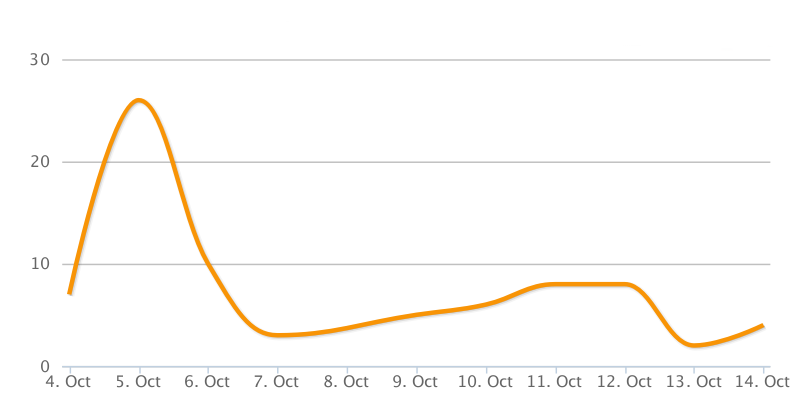
\includegraphics[width=1\linewidth]{Images/FirstSearch_QuantumTechnology.png}
   \caption{} 
 \end{subfigure}

 \begin{subfigure}[b]{0.9\textwidth}
   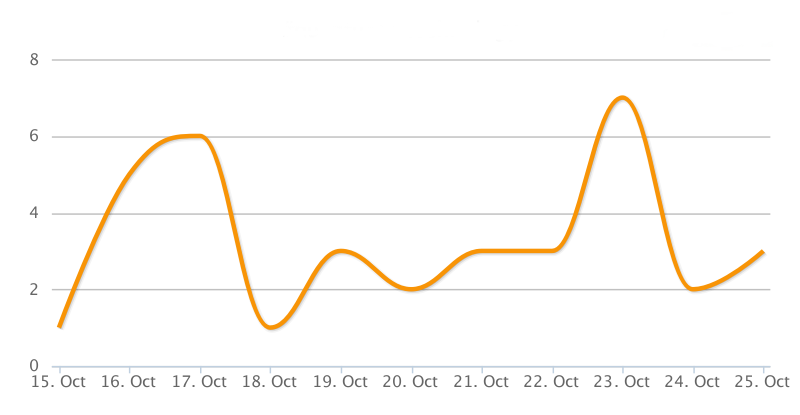
\includegraphics[width=1\linewidth]{Images/SecondSearch_QuantumTechnology.png}
   \caption{}
 \end{subfigure}
 \caption{(a) Number of tweets with hashtags \#quantum and \#technology posted between 4th and 14th October 2017. (b) As for (a) but over the time period between 15th and 25th October 2017.} 
 \label{First-SecondSearch_QuantumTechnology}
\end{figure}

\section{HPC Hashtag performance}
An analysis similar to the one outlined in section ... was conducted. The goal was to collect data to estimate the potential of QT projects. The considered hashtags were \#HPC and \#exascale. For both hashtags, the two considered time periods covered the dates from 4th to 14th and from 15th to 25th October 2017, respectively. 

The time distribution of tweets mentioning the considered keywords are shown in figures \ref{First-SecondSearch_HPC} and \ref{First-SecondSearch_Exascale}. As shown in the figures, the hashtag \#HPC is mentioned in hundreds of tweets per day, whereas \#exascale in, typically, few tens of tweets. 

The potential reach of FET projects on HPC is summarised by data in Tables . Things are discussed in section ... .

\begin{table}[t]
 \begin{center}
 
  \begin{tabular}{cccc}
   \hline 
   \hline
   \multicolumn{4}{c}{\#HPC}\\
   \hline
   \hline
   Time period & Tweets & Users & Potential Reach \\ 
   \hline
   4 - 14 Oct 2017 & 2 857 & 1 372 & 11 533 160  \\
   20 - 25 Oct 2017 & 3 015 & 1 475 & 13 315 746  \\
   \hline
   \hline
  \end{tabular}

  \bigskip

  \begin{tabular}{cccc}
   \hline 
   \hline
   \multicolumn{4}{c}{\#exascale}\\
   \hline 
   \hline
   Time period & Tweets & Users & Potential Reach \\ 
   \hline
   4 - 14 Oct 2017 & 202 & 129 & 747 846 \\
   15 - 25 Oct 2017 & 207 & 164 & 1 386 972  \\
   \hline
   \hline
  \end{tabular}
 \end{center} 
 \caption{Summary of the Twitter analytics for the hashtags \#HPC AND \#exascale over the two monitored time periods. The potential reach is defined as the total aggregate number of followers of the people who mentioned the considered keyword in their tweets.}
\label{Summary_HPC-Exascale} 
\end{table}    

\begin{figure}
 \centering
 \begin{subfigure}[b]{0.9\textwidth}
   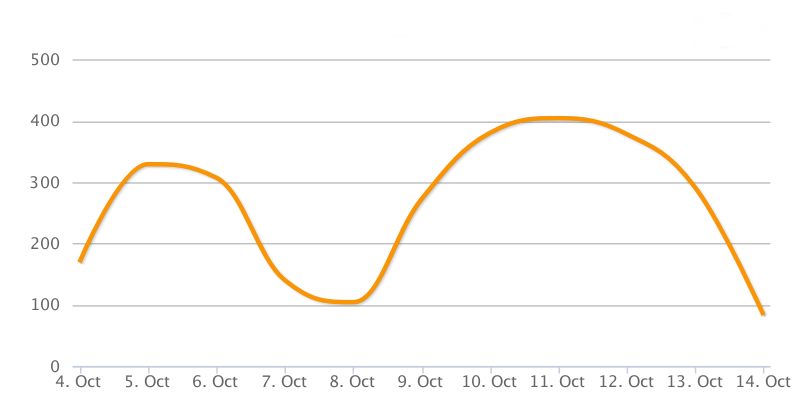
\includegraphics[width=1\linewidth]{Images/FirstSearch_HPC.png}
   \caption{} 
 \end{subfigure}

 \begin{subfigure}[b]{0.9\textwidth}
   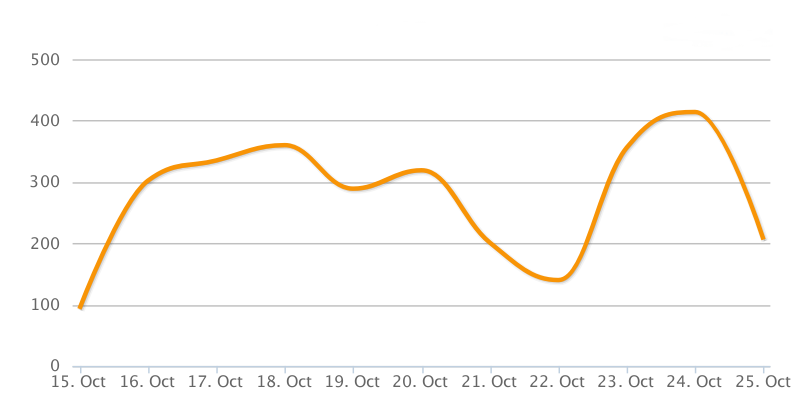
\includegraphics[width=1\linewidth]{Images/SecondSearch_HPC.png}
   \caption{}
 \end{subfigure}
 \caption{(a) Number of tweets with hashtag \#HPC posted between 4th to 14th October 2017. (b) As for (a) but over the time period between 15th and 25th October 2017.} 
 \label{First-SecondSearch_HPC}
\end{figure}

\begin{figure}
 \centering
 \begin{subfigure}[b]{0.9\textwidth}
   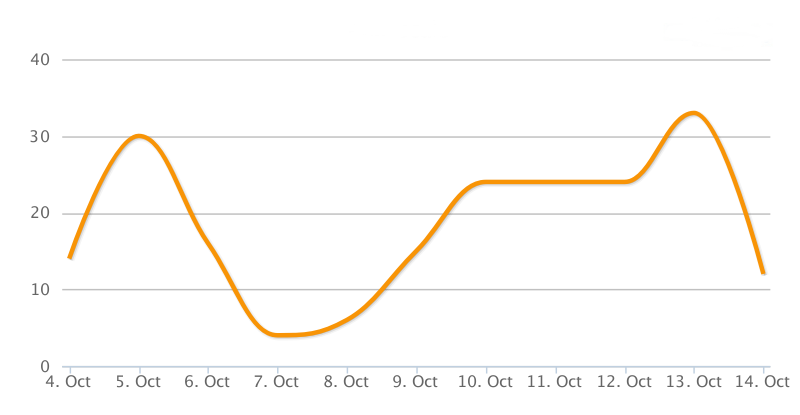
\includegraphics[width=1\linewidth]{Images/FirstSearch_Exascale.png}
   \caption{} 
 \end{subfigure}

 \begin{subfigure}[b]{0.9\textwidth}
   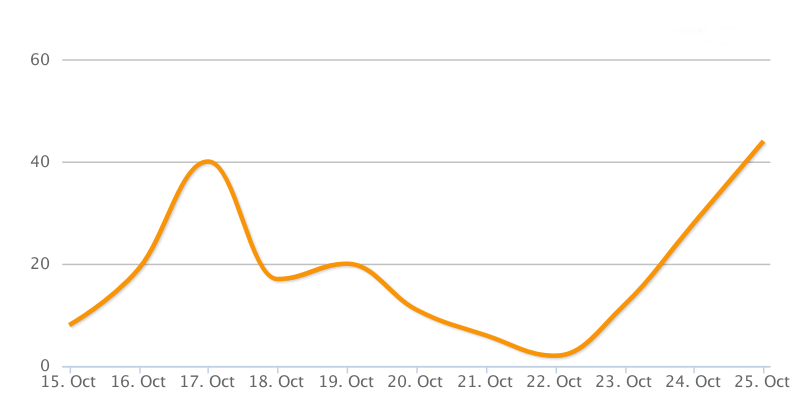
\includegraphics[width=1\linewidth]{Images/SecondSearch_Exascale.png}
   \caption{}
 \end{subfigure}
 \caption{(a) Number of tweets with hashtag \#exascale posted between 4th to 14th October 2017. (b) As for (a) but over the time period between 15th and 25th October 2017.} 
 \label{First-SecondSearch_Exascale}
\end{figure}